% TODO: Add jolly jumpers here somewhere
% TODO: Write comments about new problems

\documentclass{beamer}


\usepackage{amssymb,amsmath}
\usepackage{graphicx}
\usepackage{url}
\usepackage{color}
\usepackage{relsize}		% For \smaller
\usepackage{url}			% For \url
\usepackage{epstopdf}	% Included EPS files automatically converted to PDF to include with pdflatex
\usepackage{pagenote}[continuous,page]

%For MindMaps
% \usepackage{tikz}%
% \usetikzlibrary{mindmap,trees,arrows}%

%%% Color Definitions %%%%%%%%%%%%%%%%%%%%%%%%%%%%%%%%%%%%%%%%%%%%%%%%%%%%%%%%%
%\definecolor{bordercol}{RGB}{40,40,40}
%\definecolor{headercol1}{RGB}{186,215,230}
%\definecolor{headercol2}{RGB}{80,80,80}
%\definecolor{headerfontcol}{RGB}{0,0,0}
%\definecolor{boxcolor}{RGB}{186,215,230}

%%% Save space in lists. Use this after the opening of the list %%%%%%%%%%%%%%%%
%\newcommand{\compresslist}{
%	\setlength{\itemsep}{1pt}
%	\setlength{\parskip}{0pt}
%	\setlength{\parsep}{0pt}
%}

%\setbeameroption{show notes on top}

% You should run 'pdflatex' TWICE, because of TOC issues.

% Rename this file.  A common temptation for first-time slide makers
% is to name it something like ``my_talk.tex'' or
% ``john_doe_talk.tex'' or even ``discrete_math_seminar_talk.tex''.
% You really won't like any of these titles the second time you give a
% talk.  Try naming your tex file something more descriptive, like
% ``riemann_hypothesis_short_proof_talk.tex''.  Even better (in case
% you recycle 99% of a talk, but still want to change a little, and
% retain copies of each), how about
% ``riemann_hypothesis_short_proof_MIT-Colloquium.2000-01-01.tex''?

\mode<presentation>
{
  % A tip: pick a theme you like first, and THEN modify the color theme, and then add math content.
  % Warsaw is the theme selected by default in Beamer's installation sample files.

  %%%%%%%%%%%%%%%%%%%%%%%%%%%% THEME
  %\usetheme{Madrid}		% No subsection
  \usetheme{AnnArbor}  % Subsection on top, no color


  %\usetheme{Antibes}
  %\usetheme{Bergen}
  %\usetheme{Berkeley}		% bem bacana - menu esquerdo
  %\usetheme{Berlin}
  %\usetheme{Boadilla}
  %\usetheme{boxes}
  %\usetheme{CambridgeUS}		% bem bacana - menu superior
  %\usetheme{Copenhagen}
  %\usetheme{Darmstadt}
  %\usetheme{default}
  %\usetheme{Dresden}
  %\usetheme{Frankfurt}
  %\usetheme{Goettingen}
  %\usetheme{Hannover}		% bem bacana - menu esquerdo
  %\usetheme{Ilmenau}
  %\usetheme{JuanLesPins}
  %\usetheme{Luebeck}
  %\usetheme{Malmoe}
  %\usetheme{Marburg}		% bem bacana - menu direito
  %\usetheme{Montpellier}
  %\usetheme{PaloAlto}		% bem bacana - menu esquerdo
  %\usetheme{Pittsburgh}
  %\usetheme{Rochester}		%bacana
  %\usetheme{Singapore}
  %\usetheme{Szeged}
  %\usetheme{Warsaw}

  %%%%%%%%%%%%%%%%%%%%%%%%%%%% COLOR THEME
  %\usecolortheme{default}		% branco, azul clarinho
  \usecolortheme{crane}		% Very yellow (ok)

  %\usecolortheme{albatross}		% azul escuro, massa
  %\usecolortheme{beetle}		% cinza, menu azul
  %\usecolortheme{dolphin}		% azul e branco, legal
  %\usecolortheme{dove}			% cinza e branco, feio
  %\usecolortheme{fly}			% todo cinza, horrível
  %\usecolortheme{lily}			% parece o default
  %\usecolortheme{orchid}		% azul e branco, ok
  %\usecolortheme{rose}			% branco e violeta-claro, bonito
  %\usecolortheme{seagull}		% cinza, feio
  %\usecolortheme{seahorse}		% nhé, meio feio
  %\usecolortheme{sidebartab}		% Azul, branco, destaque na tab, interessante
  %\usecolortheme{structure}		% bichado
  %\usecolortheme{whale}		% Azul e branco, bem bonito

  %%%%%%%%%%%%%%%%%%%%%%%%%%%% OUTER THEME
  \useoutertheme{default}
  %\useoutertheme{infolines}
  %\useoutertheme{miniframes}
  %\useoutertheme{shadow}
  %\useoutertheme{sidebar}
  %\useoutertheme{smoothbars}
  %\useoutertheme{smoothtree}
  %\useoutertheme{split}
  %\useoutertheme{tree}

  %%%%%%%%%%%%%%%%%%%%%%%%%%%% INNER THEME
  \useinnertheme{circles}
  %\useinnertheme{default}
  %\useinnertheme{inmargin}
  %\useinnertheme{rectangles}
  %\useinnertheme{rounded}

  %%%%%%%%%%%%%%%%%%%%%%%%%%%%%%%%%%%

  \setbeamercovered{invisible} % or whatever (possibly just delete it)
  % To change behavior of \uncover from graying out to totally
  % invisible, can change \setbeamercovered to invisible instead of
  % transparent. apparently there are also 'dynamic' modes that make
  % the amount of graying depend on how long it'll take until the
  % thing is uncovered.

}


% Get rid of nav bar
\beamertemplatenavigationsymbolsempty

% Use short top
%\usepackage[headheight=12pt,footheight=12pt]{beamerthemeboxes}
%\addheadboxtemplate{\color{black}}{
%\hskip0.5cm
%\color{white}
%\insertshortauthor \ \ \ \
%\insertframenumber \ \ \ \ \ \ \
%\insertsection \ \ \ \ \ \ \ \ \ \ \ \ \ \ \ \ \  \insertsubsection
%\hskip0.5cm}
%\addheadboxtemplate{\color{black}}{
%\color{white}
%\ \ \ \
%\insertsection
%}
%\addheadboxtemplate{\color{black}}{
%\color{white}
%\ \ \ \
%\insertsubsection
%}

% Insert frame number at bottom of the page.
% \usefoottemplate{\hfil\tiny{\color{black!90}\insertframenumber}}

%% makes the ppagenote command for figure references at the end.

\usepackage[english]{babel}
%qq\usepackage[latin1]{inputenc}
\usepackage{CJKutf8}
\usepackage{subfigure}

\usepackage{times}
\usepackage[T1]{fontenc}

\makepagenote
\renewcommand{\notenumintext}[1]{}
\newcommand{\ppagenote}[1]{\pagenote[Page \insertframenumber]{#1}}

\title[Programming Challenges]{GB20602 - Programming Challenges}
\author[Claus Aranha]{Claus Aranha\\{\footnotesize caranha@cs.tsukuba.ac.jp}}
\institute[U. Tsukuba]{University of Tsukuba, Department of Computer Sciences}


\usepackage[normalem]{ulem}

\title[]{GB21802 Programming Challenges}
\subtitle[]{Week 2 - Sorting Algorithms}
\author[Claus Aranha]{Claus Aranha\\{\footnotesize caranha\@@cs.tsukuba.ac.jp}}
\institute{College of Information Sciences}
\date{2015-04-20\\{\tiny Last updated \today}}

%\thanks{fcampelo@ufmg.br}

\begin{document}

\section{Outline}
\subsection{Outline}

\begin{frame}
\maketitle
\end{frame}

\begin{frame}
  \frametitle{Notes: Week 1 submissions results}
  \begin{itemize}
    \item 3n+1:
    \item Chess:
    \item Erdos:
    \item Scoreboard:
  \end{itemize}

  \begin{alertblock}{Important note}
    The system just stores your \structure{First submitted code}. If
    you want to send a new version after that, you have to
    \structure{e-mail me}. Sorry about that.
  \end{alertblock}
\end{frame}

\subsection{Introduction}

\begin{frame}
  \frametitle{The importance of Sorting}
  \begin{block}{Sorting}
    Given a collection of items, change the position of those items
    inside the collection so that they obey some pre-defined order
    (alphabetical order, numerical order, etc)
  \end{block}
  \vfill
  \begin{center}
    Why is sorting important?
  \end{center}
  \begin{itemize}
    \item Sorting the data is the first step of many well known
      algorithms;
    \item Sorting can also speed up some other algorithms;
    \item Sorting is a good way to start learning about Computer
      Science theoretical research;
  \end{itemize}

\end{frame}

\begin{frame}
  \frametitle{The importance of Sorting (2)}

\begin{center}
  Even Bill Gates has published a paper on Sorting!
  \medskip
  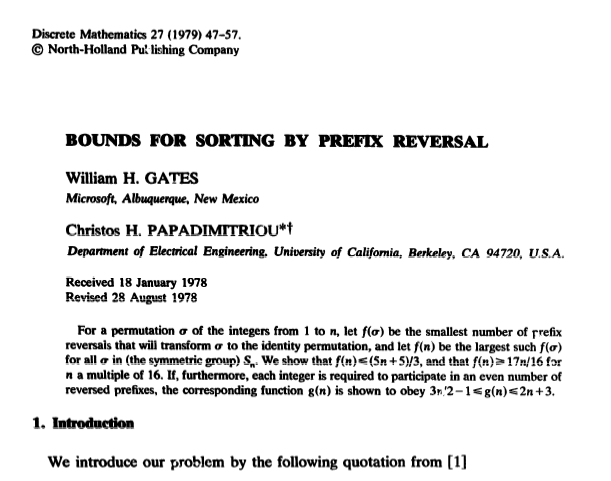
\includegraphics[width=0.7\textwidth]{img/billgates}
\end{center}
\end{frame}

\section{Sorting}
\subsection{Sorting Applications}
\begin{frame}
  \frametitle{Sorting Applications} 

  Sorting can be used as a step in a huge number of algorithms. Let us
  check a few of them. Please give your own suggestions as well!
\end{frame}


\begin{frame}
  \frametitle{Sorting Applications (1)}
  \begin{block}{Testing for Uniqueness or Duplicates}
    After sorting a data array, any duplicate data will be near each
    other. You can test for the existence of duplicates using only one pass
    through the array.
  \end{block}

  \begin{onlyenv}<2>
    \begin{block}{Unique subset}
      Using the same idea as above, you can find the largest subset of
      unique items, by keeping track of any unique items (or row of items)
      in a different array.
    \end{block}

    \begin{block}{Frequency Counting, Finding the Mode}
      Using the same idea as above, you can count the frequency of a
      value (by counting duplicates). The value with the highest
      number of duplicates is the \emph{Mode}. 
    \end{block}
  \end{onlyenv}
\end{frame}


\begin{frame}
  \frametitle{Sorting Applications (2)}
  \begin{block}{Finding the Median, or a quantile}
    You can find the $n^{th}$ largest (smallest) element by sorting an
    array, and picking the $n^{th}$ element in the sorted array.

    The median is the element in the half of the array (different from
    the mean!).
  \end{block}
  
  \begin{block}{Prioritizing Events}
    We can sort events by priority (or by the time they should
    happen). And now we have a priority queue.
  \end{block}

  \begin{block}{Finding a target pair}
    We want to find $a$ and $b$ so that $a+b=z$. After finding the
    lowest value $x$ in the array, we find $y$ so that $z - x = y$,
    and we do the search from both ends.
  \end{block}
\end{frame}

\begin{frame}
  \frametitle{Sorting Applications (3)}
  Can you give me suggestions of other uses for sorting?
\end{frame}


\subsection{Too many algorithms!}

\begin{frame}
  \frametitle{How many sorting Algorithms are there?}
  \begin{columns}[c]
    \column{0.5\textwidth}
    {\tiny
    \begin{itemize}
    \item bubblesort
    \item insertion sort
    \item selection sort
    \item heapsort
    \item mergesort
    \item quicksort
    \item radix sort
    \item bin sort
    \item Shell sort
    \item gnome sort
    \item library sort
    \item comb sort
    \item tree transversal
    \item sorting networks
    \item cocktail shaking sort
    \item bucket sort
    \item bogo sort
    \item bitonick sort
    \item ...
    \item And many more!
    \end{itemize}}
    \column{0.5\textwidth}
    \includegraphics<2>[width=1\textwidth]{img/fliptable}
  \end{columns}
\end{frame}

\begin{frame}
  \frametitle{Why are there so many sorting algorithms?}
  \begin{itemize}
  \item Theoretical research in sorting can give insights about the
    theoretical basis of other algorithms;
    \bigskip
  \item Some of these algorithms are very efficient in very specific
    situations;
    \bigskip
  \item Sometimes you can exchange memory for time complexity, or
    vice-versa;
  \end{itemize}
\end{frame}

\begin{frame}
  \frametitle{Why are there so many sorting algorithms?}
  \begin{center}
    For example, the Bill Gates Paper...
  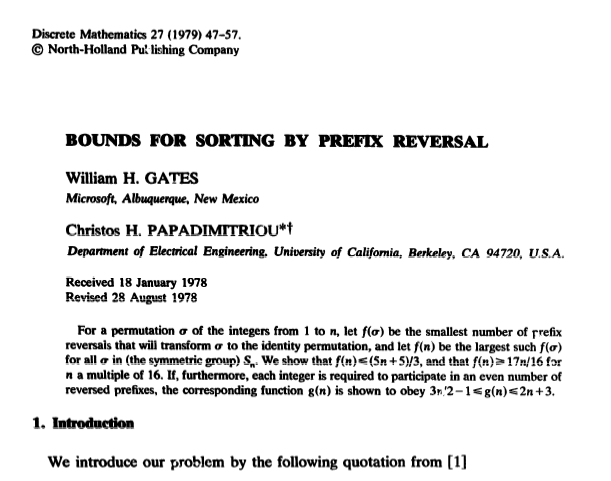
\includegraphics[width=0.5\textwidth]{img/billgates}
  \end{center}
  \medskip
  {\small It focuses on sorting by ``reverse radix'' -- an operation that
  reverses a sub-array. This is very important to calculate the
  genetic distance between two individuals. (How many reverse
  operations does it take to go from individual A to individual B?)}
\end{frame}

\subsection{Characteristics of Sorting Algorithms}

\begin{frame}
  \frametitle{Characteristics of sorting algorithms}
  \begin{block}{Computational Complexity}
    \begin{itemize}
    \item \structure{How many comparisons?} Comparisons require
      conditionals in the machine code, and sometimes can be,
      themselves, very expensive.
    \item \structure{How many swaps?} Moving memory around can also be
      expensive, depending on how much memory we are using for the
      data (Main memory, cache, etc).
    \item \structure{Memory Requirements:} Some algorithms require an
      extra array, or maybe even more memory, in exchange for a
      reduced number of comparisons/swaps.
    \end{itemize}
  \end{block}
\end{frame}

\begin{frame}
  \frametitle{Characteristics of sorting algorithms}
  \begin{columns}[c]
    \column{0.7\textwidth}
    \begin{itemize}
    \item \structure{Stable Algorithms} guarantee that two objects who
      are ``equal'' in the sorting order will maintain their relative
      position after sorting.
    \item \structure{Unstable Algorithms} do not guarantee the final
      order of two objects who are ``equal'' in regard to the sorting
      comparison function.
    \item (for example, two objects containing the same data, but
      different memory addresses)
      \medskip
    \end{itemize}
    \column{0.3\textwidth}
    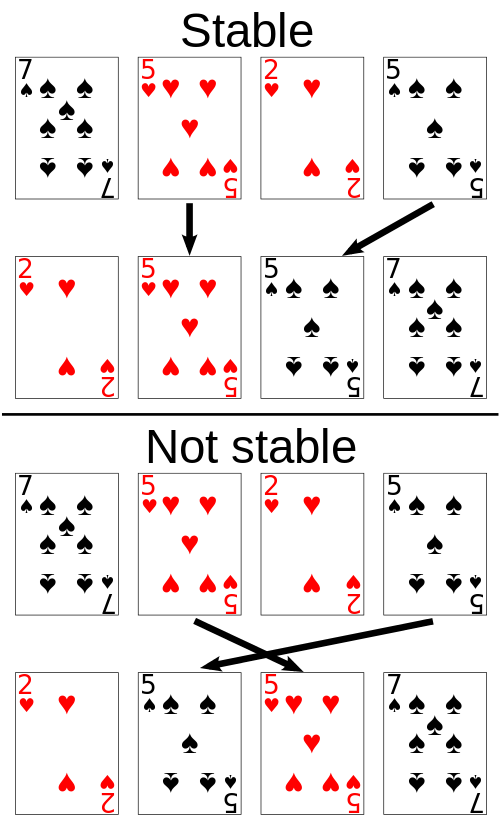
\includegraphics[width=0.9\textwidth]{img/sortingstability}
  \end{columns}
\end{frame}

\begin{frame}
  \frametitle{Characteristics of sorting algorithms}
    Other questions:
    \begin{itemize}
    \item Is the algorithm parallelizable?
    \item Is the algorithm recursive? How complex is the code?
    \item Is the algorithm based on comparisons, or on hashes?
    \end{itemize}
\end{frame}


\section{Algorithm Review}
\subsection{Sorting Algorithm Review}

\begin{frame}
  \frametitle{Sorting Algorithm Review}
  \begin{center}
    Let us review quickly some sorting algorithms
  \end{center}
\end{frame}

\begin{frame}[fragile,singleslide]
  \frametitle{Selection Sort}
  \begin{block}{}
{\smaller
\begin{verbatim}
Divide data into sorted list and unsorted list;
For i = 1 to length of data:
    Select lowest element in unsorted list;
    Move selected element to the end of sorted list;
\end{verbatim}
}
  \end{block}

\begin{itemize}
\item Selection sort performs many comparisons, but few data swaps;
\item Normally, it is \alert{very inneficient}. But if you use the
  correct data structure for the unsorted data, it becomes the
  \structure{very efficient} heapsort!
\end{itemize}
\end{frame}

\begin{frame}[fragile,singleslide]
  \frametitle{Merge Sort}
  \begin{block}{}
{\smaller
\begin{verbatim}
If data size is < 3:
    sort data;
Else:
    Mergesort(first half)
    Mergesort(second half)
    Merge(first half, second half)
\end{verbatim}
}
  \end{block}
  \begin{itemize}
  \item The mergesort can be easily parallelized. You can sort HUGE
    amounts of data efficiently in a parallel context;
  \item In fact, it is implemented in many standard libraries;
  \item How would you implement it without recursion?
  \end{itemize}
\end{frame}

\begin{frame}[fragile,singleslide]
  \frametitle{Quick Sort}
  
  \begin{block}{}
{\tiny
\begin{verbatim}
Quicksort (dataarray):
  While dataarray > 1:
    p = Partition(dataarray);
    Quicksort(dataarray[:p-1]);
    Quicksort(dataarray[p+1:]);

Partition (d):
  Select a Pivot;
  PivPlace = 1;
  for i in d:
    if d[i] < Pivot:
       place d[i] in PivPlace;
       PivPlace++;
  place Pivot in PivPlace;
  return PivPlace;
\end{verbatim}
}
\end{block}

  \begin{itemize}
  \item Quicksort is well known, because it is very fast in the average case.
  \item In the worst case, quicksort is actually slow (can you build a worst case?)
  \item Performance is heavily dependent of the smart selection of a
    pivot. Random pivots are usually an ``okay'' choice.
  \end{itemize}
\end{frame}

\begin{frame}[fragile,singleslide]
  \frametitle{Bucket Sort}

  \begin{block}{}
    {\smaller
\begin{verbatim}
Create k Buckets;
For each element in data:
  Place element in correct bucket;
For i = 1 to k-1:
  Concatenate bucket i to bucket i+1;
\end{verbatim}
}
  \end{block}
  \bigskip

  \begin{itemize}
  \item Can sort in O(n+k) -- linear!
  \item However, the price to pay is the size of $k$;
  \item If you know the ``absolute'' positioning of the data, and
    there are many repetitions, $k$ will be very 
  \item On the other hand, for ``infinite'' data values, $k$ can also get infinite!
  \item This method is not based on comparisons!
  \end{itemize}
  % Bucket Sort
\end{frame}

\section{Relaxing}
\subsection{Relax Time}

\begin{frame}
  \frametitle{Sorting Methods Video}
  Movie time! Can you identify the sorting methods?
  \vfill
  
  Why does the C++ sort leave ``dirt'' to be cleaned in the last pass?
\end{frame}


\begin{frame}
  \frametitle{Bogo Sort}
  \begin{block}{The Worst Sorting Algorithm}
    \begin{enumerate}
      \item Shuffle the Data
      \item If the data is not sorted, return to 1
    \end{enumerate}
  \end{block}
  \bigskip
  
  \begin{itemize}
  \item Calculate the complexity of this Algorithm!
  \item Will this algorithm always stop?
  \end{itemize}
\end{frame}

\begin{frame}
  \frametitle{The \alert{Quantum} Bogo Sort}
  
  \begin{block}{The \alert{Best} Sorting Algorithm}
    \begin{enumerate}
    \item Shuffle all the data;)
    \item Check if the data is sorted;
    \item If the data is not sorted, destroy the entire universe.      
    \end{enumerate}
  \end{block}
\end{frame}

\section{Using Sorting}

\subsection{Using Sorting}

\begin{frame}
  \frametitle{Sorting in Programming Challenges}
  \begin{block}{}
    Your language libraries have already implemented some sorting for
    you. You will often want to use that.
  \end{block}
  \medskip
  \begin{itemize}
    \item \structure{Java:} Collections.sort()
    \item \structure{C (stdlib.h):} qsort();
    \item \structure{C++ (stl):} sort(), stable\_sort; 
  \end{itemize}
  \medskip
  You usually have to implement the comparison function, except in
  trivial cases.
\end{frame}

\begin{frame}
  \frametitle{Implementing Sorting Functions}
  \begin{block}{Sorting on multiple attributes of your data}
    Sort by height (ascending), in case of tie sort by last name
    (alphabetical), in case of tie sort by weight (descending), in
    case of tie sort by who has the birthday closest to June 30th.
  \end{block}
  \begin{center}
    How do you do that?
  \end{center}
\end{frame}

\begin{frame}
  \frametitle{Implementing Sorting Functions (2)}
  \begin{block}{Sorting on multiple attributes of your data}
    Sort by height (ascending), in case of tie sort by last name
    (alphabetical), in case of tie sort by weight (descending), in
    case of tie sort by who has the birthday closest to June 30th.
  \end{block}
  \medskip
  \begin{itemize}
  \item<1> Multiple Passes: Sort the items by the least important
    criteria, then by the next least important criteria, and so
    on. Simple, a bit slow, requires a stable sorting algorithm.
  \item<2> Single Pass: Make a complex comparison function that takes
    all the sorting conditions into account. Faster than multiple
    passes, but be careful with code complexity!
  \item<3> Pre-process the data: In some cases, you can modify parts
    of the data to make sorting simple. Example: ``Sort closest to X''
    = sort ``abs(X-value)'';
  \end{itemize}
\end{frame}

\section{This Week's Problems}

\subsection{Problem}
\begin{frame}
  \begin{itemize}
  \item Crypt Kicker II
  \item File Fragmentation
  \item Vito's Family
  \item \sout{Football (aka Soccer)} <- \alert{Don't do this one!}
  \item Shoemaker's Problem
  \end{itemize}
\end{frame}
\end{document}
